\documentclass[a4paper,twoside,12pt]{book}
\usepackage[T1]{fontenc} 
\usepackage[utf8]{inputenc}   
\usepackage[czech]{babel} 
%\usepackage[a4paper, hmarginratio=3:2]{geometry} 
\usepackage[a4paper, inner=3.5cm, textwidth=15cm, top=2.5cm, textheight=24cm]{geometry} 
\usepackage{pdfpages} % pokud nemáte formulář "Zadání bak./dipl. práce" naskenovaný jako PDF, tak ZAKOMENTUJTE
\usepackage[hidelinks]{hyperref} % v PDF budou klikací odkazy ("hidelinks" je nebude rámovat)

\usepackage{graphicx} 
\usepackage{epsfig} 
\usepackage{float} 
\usepackage{caption} 
\usepackage{tabularx} 
\usepackage{listings}  
\usepackage{amsmath} 
\usepackage{cite}

\frenchspacing % za~větou bude mezislovní mezera (v anglických textech je mezera za~větou delší)
\widowpenalty=1000 % "síla" zákazu vdov (= jeden řádek ze~začátku odstavce na~konci stránky)
\clubpenalty=1000 % "síla" zákazu sirotků (= jeden řádek/slovo z konce odstavce samostatně na~začátku stránky)
\brokenpenalty=1000 % "síla" zákazu zlomu stránky za~řádkem, který má na~konci rozdělené slovo


\usepackage{parskip}
%\usepackage{indentfirst}
\pagenumbering{arabic} % číslování stránek arabskými číslicemi
\pagestyle{plain}      % stránky číslované do~le uprostřed

%----------------------------------------------------------------------------------------
%	TITLE SECTION
%----------------------------------------------------------------------------------------

\newcommand{\horrule}[1]{\rule{\linewidth}{#1}} % Create horizontal rule command with 1 argument of height

\newcommand{\cvut}{ČESKÉ VYSOKÉ UČENÍ TECHNICKÉ
V~PRAZE}
\newcommand{\nazevcz}{Elektronové dělo a detekce elektronového svazku}
\newcommand{\fjfi}{Fakulta jaderná a fyzikálně inženýrská}
\newcommand{\kf}{Katedra Fyziky} 
\newcommand{\logoCVUT}{
\includegraphics{symbol_cvut_konturova_verze_cb.pdf}}



\begin{document}
%\nocite{*}

\newpage 
\thispagestyle{empty}

\begin{center}
	{\LARGE
		\cvut\par
		\fjfi
	}
    \vspace{10mm}

   \vspace{10mm} \logoCVUT \vspace{15mm} 

   {\huge \textbf{\nazevcz}\par}
   
   \vspace{15mm}
   
   Ekaterina Eremenko, Anežka Kabátová, Jakub Kubát, \\
Tomáš Novák, Monika Robotková, Jaroslav Štorek, \\
Tomáš Truhlář, Matěj Vaculčiak

\vspace{15mm}

\normalsize\today

\end{center}


\newpage 
\thispagestyle{empty}

{\Large
	\textbf{Členové kolaborace}
}

\vspace{5mm}

\begin{center}
\textbf{Koordinátor projektu} \\
Tomáš Truhlář 

    \vspace{5mm}
    
\textbf{Mluvčí projektu} \\
Anežka Kabátová \\

\vspace{3mm}

***

\vspace{3mm}

\textbf{Konstrukce elektronového děl}a \\
Monika Robotková\\
Jaroslav Štorek\\
Tomáš Novák\\
Tomáš Truhlář

   \vspace{5mm}
   
\textbf{Fokusace elektronového svazk}u \\
Ekaterina Eremenko\\
Jakub Kubát


\vspace{5mm}

\textbf{Měření elektronového svazku} \\
Anežka Kabátová \\
Matěj Vaculčiak


\end{center}

\newpage  
\parskip=0pt
\tableofcontents 
\parskip=7pt
\newpage 
\listoffigures
\newpage
\listoftables
\newpage

\newpage

\newpage
\chapter*{Úvod} % normalni kapitola \chapter{kapitola}
\addcontentsline{toc}{chapter}{Úvod}

Za úkol na předmětu Projektové Praktikum bylo zadáno navrhnout a následně sestrojit aparaturu pro urychlování svazku elektronů a zařízení pro jejich detekci, což zahrnuje návrh a realizaci zapojení elektronového děla, zdroje vysokého napětí, doplňující soustavu fokusující svazek a v neposlední řadě samotný detektor intenzity elektronového svazku. 

Hned v úvodu jsme se tedy rozdělili na tři podskupiny, z nichž jedna se zabývala samotnou konstrukcí děla, jeho instalací do vakuové komory a zprovozněním urychlovací soustavy. Druhá skupina se zaměřila na fokusaci svazku elektronů, která spočívala v nalezení ideální konfigurace fokusovacích diod na základě simulací v programu SIMION. Třetí skupina se zabývala výrobou detektoru pro měření intenzity elektronového svazku, připojení vyčítacího zařízení a následné zpracování a analýza naměřených dat.

Na začátku projektu jsme se rozhodli, že se pokusíme vytvořit elektronový svazek o energii zhruba 80 keV, aby bylo možné použít monolitický pixelový detektor, který jsme si byli schopni sami sestrojit. První pokusy vytvořit elektronový svazek se žhaveným wolframovým vláknem jako zdrojem elektronů však nebyly úspěšné a později jsme přešli k průmyslovému elektronovému dělu. Svazek jsme urychlovali měděnými elektrodami. Z důvodu pozorovaných elektrických výbojů jsme nebyli na elektrodách schopni dosáhnout zamýšleného potenciálového rozdílu 80 kV, nýbrž jen 18 kV. K detekci signálu jsme proto použili destičku ze slitiny mědi a zlata, která konvertovala elektrony na námi detekovatelné fotony, a analyzovali výsledek měření.

První kapitola poskytuje teoretický úvod o elektronech a jejich chování v prostředí se sníženým tlakem. Je zde také popsán princip katodového záření a možnosti vedení elektrického proudu ve vakuu. 

Druhá kapitola pojednává o základních principech vzniku elektrických výbojů a jejich dělením. Druhá část této kapitoly se věnuje problematice vzniku elektrických výbojů v našem experimentu a popisuje způsoby, kterými jsme se snažili výbojům zamezit a předejít.

Třetí kapitola se zabývá principem fungování elektronového děla a emisí elektronů. Dále je zde popsáno sestavení vlastního elektronového děla a jeho technické parametry.

Ve čtvrté kapitole je představen zdroj elektronů ES40-PS, kterým bylo v pozdější fázi projektu nahrazeno naše původní elektronové dělo. V kapitole jsou rozepsány především technické detaily tohoto zdroje a jeho správné ovládání.

Pátá a šestá kapitola jsou věnovány fokusaci elektronového svazku. První ze zmiňovaných kapitol se zabývá především teorií samotné fokusace. Druhá zmíněná kapitola pak představuje simulační program SIMION a jeho konkrétní využití v našem experimentu.

Předposlední kapitola popisuje principy detekce elektronů a představuje detektor použitý v našem experimentu, jeho výrobu a technické parametry.

V poslední kapitole je uvedena metodika měřením, naměřená data a výsledky analýzy dat.



\newpage
\chapter{Elektrické výboje}
\par Při přípravě elektronového svazku jsme se snažili, aby byl dostatečně energetický pro dosažení prahu detekce použitého detektoru. Proto jsme cílili na dosažení elektronového svazku o energii zhruba 80 keV. Urychlení jsme prováděli pomocí rozdílu elektrického potenciálu na měděných elektrodách použitím zdrojů kladných pólů napětí. 
\par K dosažení zamýšlené energie elektronového svazku jsme použili zdroj vysokého napětí (HV) s rozsahem až do 100 kV a dva zdroje o maximálním rozsahu 5 kV. Experiment jsme prováděli ve vakuové komoře. U průchodky do vakuové komory jsme však nebyli schopni elektrody od sebe izolovat z důvodu špatné přístupnosti, takže jak z vnitřní, tak z vnější strany byla vzdálenost mezi elektrodami menší než jeden centimetr. V tomto místě hrozilo, že dojde k elektrickému výboji.

\section{Teorie elektrického výboje}
\par Základním dělením elektrických výbojů je dělení na samostatné a nesamostatné \cite{kracik}. Nesamostatné výboje jsou vázány na vnější (tzv. ionizační) činidlo, bez kterého nemohou probíhat. Ionizačním činidlem mohou být například elektrony vystupující ze žhavené katody nebo ozařování výbojového prostoru rentgenovými paprsky. Pokud se výboj může udržet, i když ionizační činidlo nepůsobí, nazýváme ho samostatným. Takovými výboji jsou výboje temné, doutnavé, obloukové, jiskrové, vysokofrekvenční a koróny. Dále rozebereme doutnavé a jiskrové výboje \cite{kracik}.

\subsection{Samostatné výboje}
\par Teorie samostatného výboje vznikla z rozšíření teorie nesamostatného výboje. Teorie nesamostatných výbojů je založena na myšlence Townsendových lavin, kdy žhavená katoda produkuje stálý počet elektronů za jednotku času, které dále ionizují částice plynu mezi elektrodami a produkují se laviny. U samostatného výboje již uvažujeme dostatečně vysoké napětí mezi elektrodami, že ionizační činidlo není zapotřebí a výboj probíhá pomocí vysokého počtu ionizací nárazem.
\par Minimální napětí na elektrodách, které je potřeba ke vzniku výboje $U_z$, tj. zápalné napětí samostatného výboje, lze podle Townsenda vypočítat jako \cite{kracik}

\begin{equation} 
U_z=A \frac{pd}{\ln \Big[ B \frac{pd}{\ln \big( 1+ \frac{1}{\eta_+} \big)} \Big]} \quad \text{,}
\label{eq:paschen}
\end{equation}

kde $A=BU_i$ a $U_i$ je ionizační napětí, $B=\frac{1}{p\lambda_e}$ je počet srážek na jednotku dráhy elektronu při jednotkovém tlaku prostředí, kde $\lambda_e$ je střední volná dráha elektronu, $p$ je tlak, $d$ je vzdálenost elektrod a $\eta_+$ charakterizuje vlastnosti materiálu katody, které ovlivňují pravděpodobnost emise elektronů z katody kladnými ionty (koeficient sekundární emise elektronů). Rovnice \eqref{eq:paschen} je nazývána Paschenovým zákonem. Bylo zjištěno, že konstanty $A$ a $B$ se nemění v oblasti $E/p=450-7500$ $\frac{\text{V}}{\text{kPa} \cdot \text{cm}}$ ($E$ je elektrická intenzita) a jsou rovny $A=2737,5$ $\frac{\text{V}}{\text{kPa} \cdot \text{cm}}$ a $B=112,5$ $\frac{\text{V}}{\text{kPa} \cdot \text{cm}}$ \cite{Husain1982}.
\par Průběh zápalného napětí různých plynů je znázorněn na Obr. \ref{obr:paschen}, specálně pro vzduch na Obr. \ref{obr:paschen_air}. Zápalné napětí $U_z$ nabývá minima v \cite{kracik}

\begin{equation}
(pd)_{min}=\frac{2,781}{B} \ln \Big( 1+ \frac{1}{\eta_+} \Big) \quad \text{.}
\end{equation}


\begin{figure}[h!]
\centering
\begin{minipage}[c]{200pt}
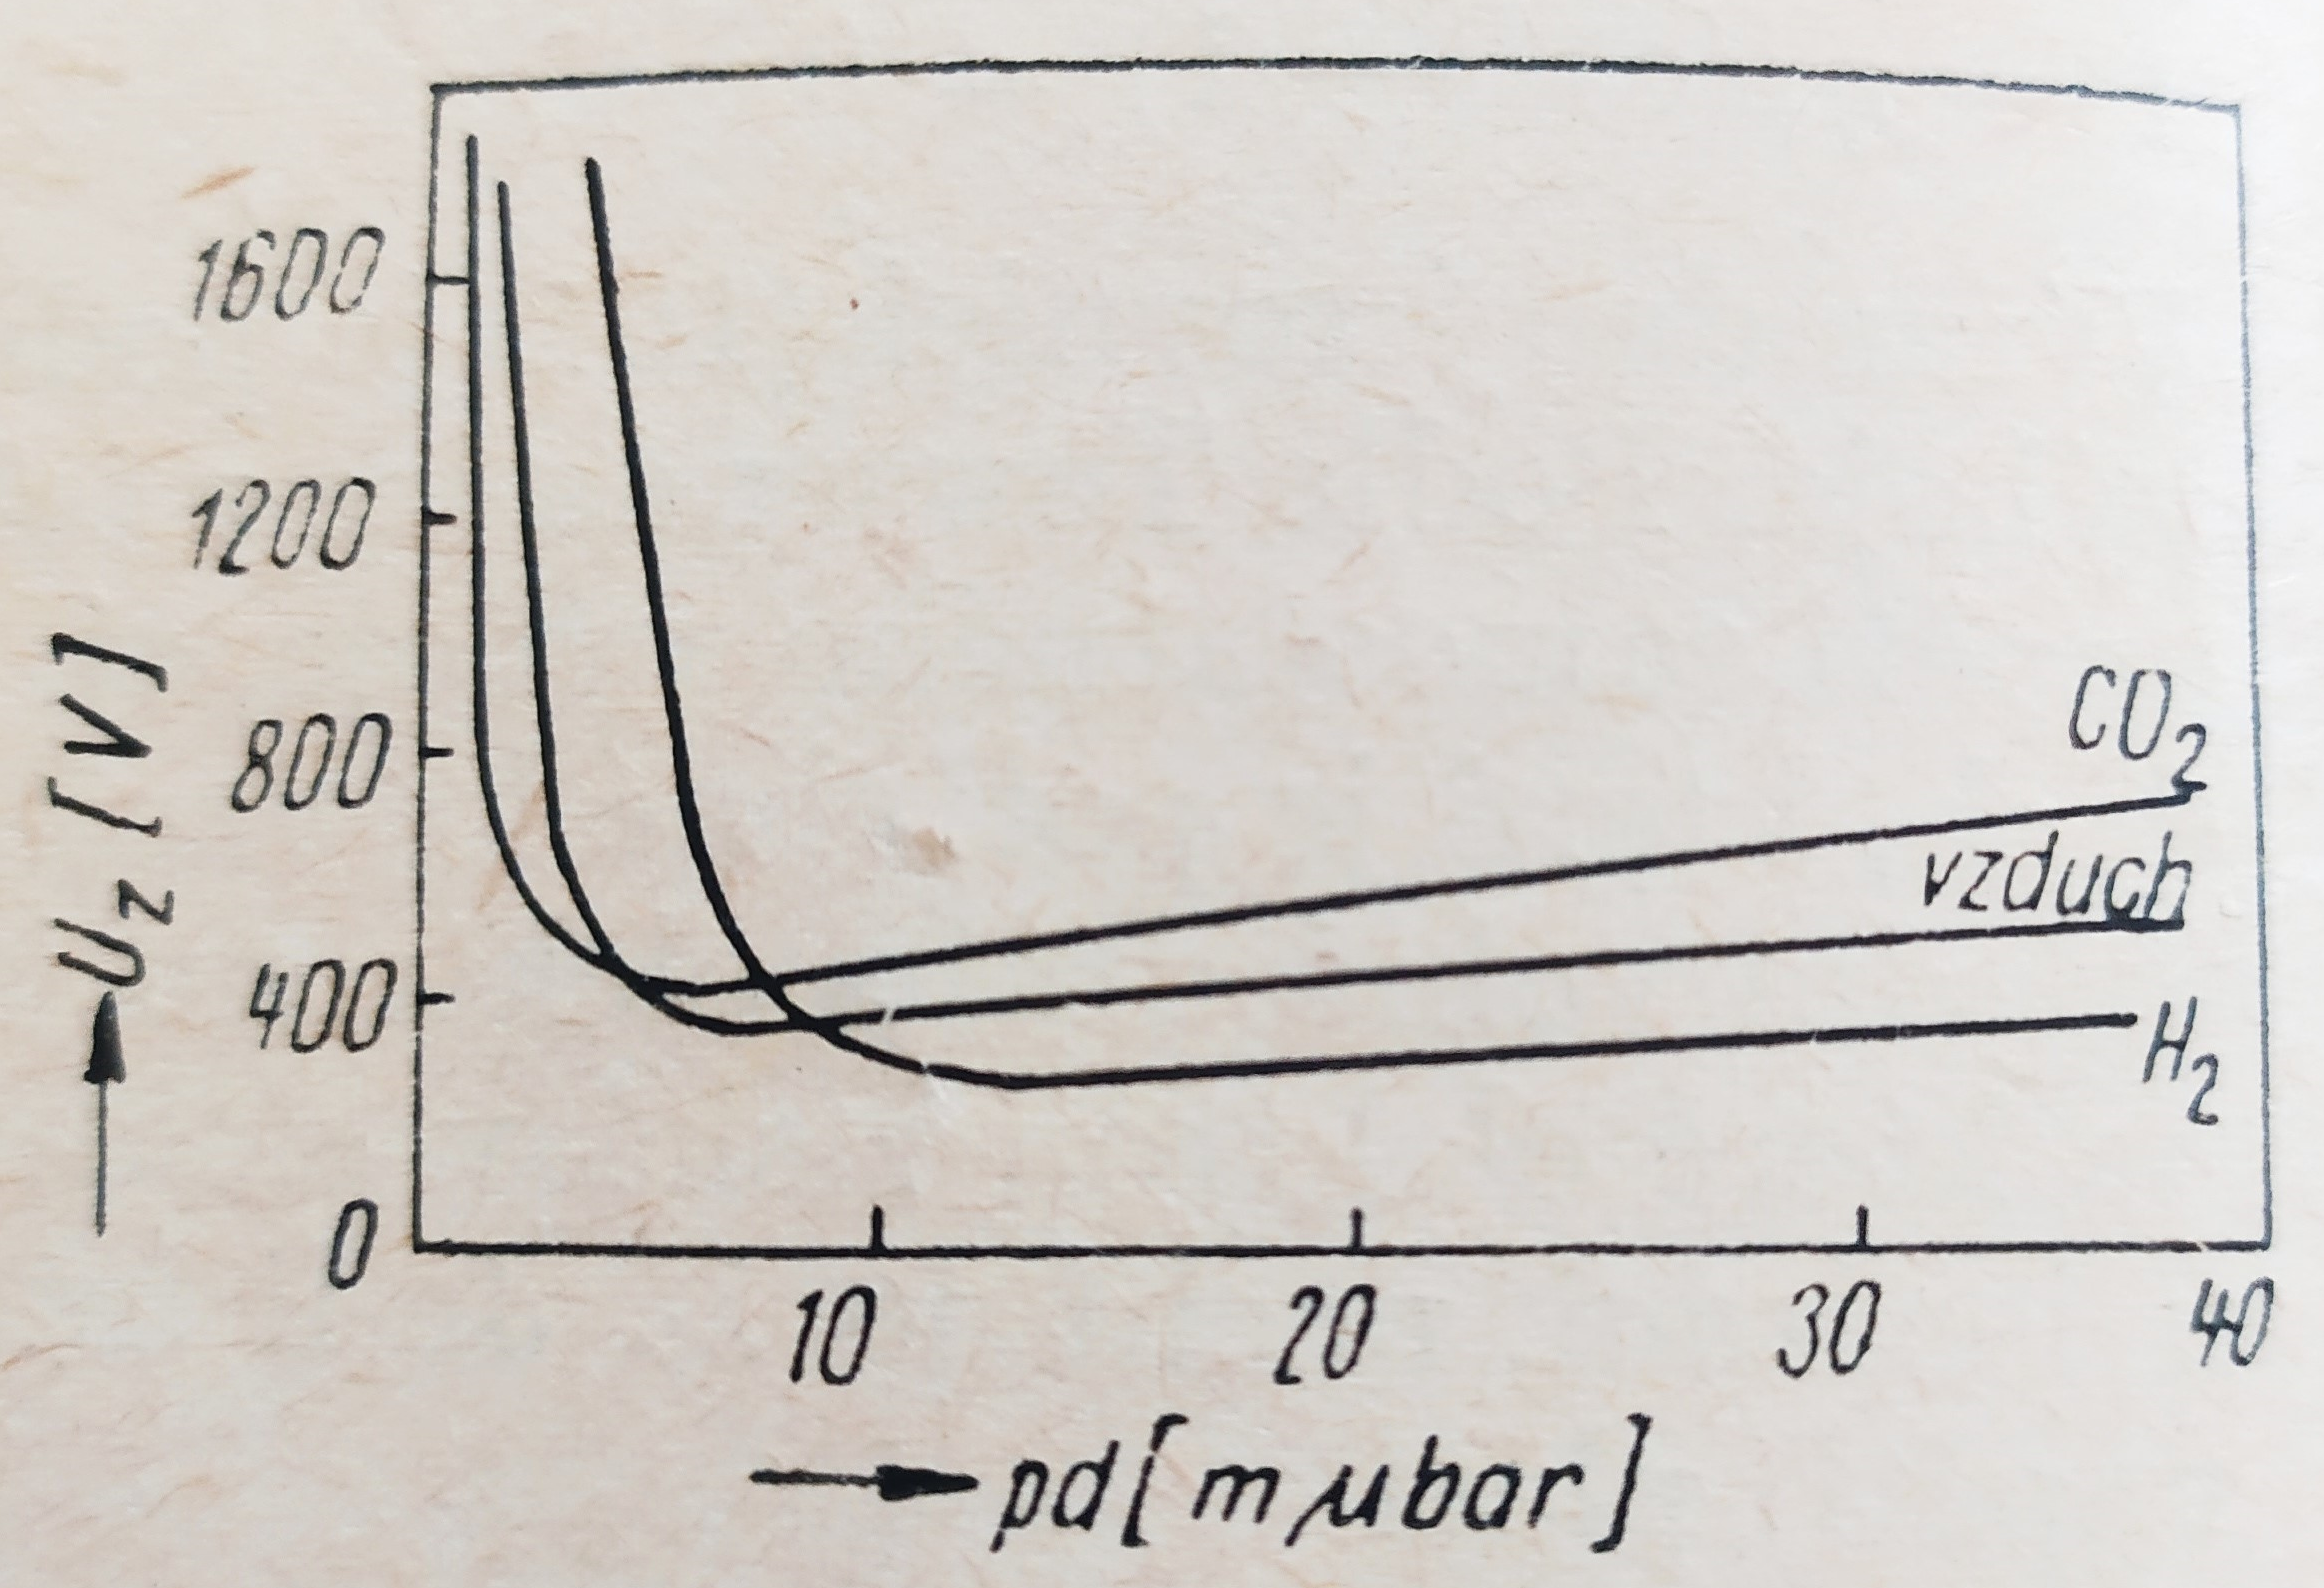
\includegraphics[width=\textwidth]{Figure/02/paschen.png}
\end{minipage}
\begin{minipage}[c]{200pt}
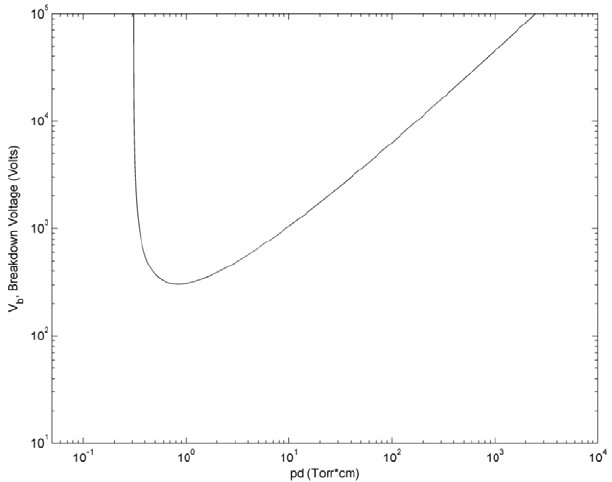
\includegraphics[width=\textwidth]{Figure/02/paschen_air.png}
\end{minipage}
\\
\begin{minipage}[c]{200pt}
\caption{Zápalné napětí různých plynů \cite{kracik}. (1~$\mu$bar = 0,1 Pa)}
\label{obr:paschen}
\end{minipage}
\begin{minipage}[c]{5pt}
\end{minipage}
\begin{minipage}[c]{200pt}
\caption{Paschenova křivka pro vzduch z roku 2011 \cite{Martins2011}. (Torr$\cdot$cm = 133 Pa$\cdot$cm)}
\label{obr:paschen_air}
\end{minipage}
\end{figure}

\subsubsection{Doutnavý výboj}
\par Přechod od nesamostatného výboje k samostatnému je doprovázeno vzrůstem proudu a světélkováním plynu. Pro doutnavý výboj jsou charakterizující světélkující oblasti především u anody, kde dochází k nejvíce srážkám elektronů s molekulami plynu \cite{kracik}. V závislosti na rozložení prostorových nábojů se průběh potenciálu mezi katodou a anodou deformuje a světélkující oblasti se nacházejí i dále od anody. Rozložení prostorových nábojů se mění i s tlakem \cite{edu-techmania}. Na Obr. \ref{obr:doutnavy} je znázorněn doutnavý výboj ve vzduchu při tlaku 100 Pa.

\subsubsection{Jiskrový výboj}
\par Jiskrový výboj je nestabilní a nestacionární forma samostatného výboje, která nevyžaduje působení ionizačního činidla \cite{kracik}. Má vzhled jasně svítících větvících se kanálů o vysoké teplotě a v plynu je doprovázen akustickými jevy. Přestože se při jiskrových výbojích uplatňuje jiný princip vzniku než při výboji lavinovém, tzv. kanálový mechanismus, platí pro ně Paschenův zákon \eqref{eq:paschen} \cite{kracik}. Jelikož se součinitel $\eta_+$ vyskytuje v Paschenově zákoně ve tvaru $\ln \ln \eta_+$, materiál katody nemá vliv na velikost $U_z$ \cite{kracik}. Zápalné napětí je nazýváno napětím průrazu a u vzduchu činí toto průrazné napětí při normání teplotě a tlaku 3 MV/m = 30 kV/cm \cite{tipler1987}.

%napočítat hodnoty napětí pro průraz s tim, že eta dáme třeba 40 podle 
%https://arxiv.org/ftp/arxiv/papers/1302/1302.2333.pdf 
%https://arxiv.org/ftp/arxiv/papers/1302/1302.2334.pdf
% dále doutnavý a jiskrový výboj a pak popis naší aparatury a co jsme pozorovali - to fialový a pak blesk, jak jsme to vyřešili (izolace nefungovala, přendání, nižší napětí)


\begin{figure}[h!]
\centering
\begin{minipage}[c]{200pt}
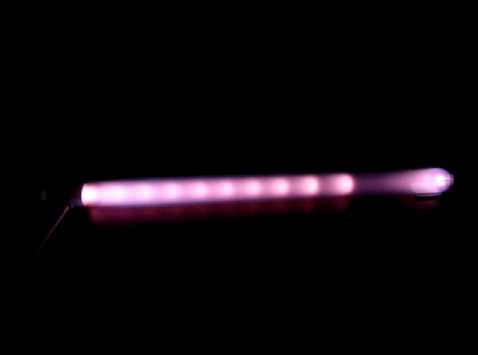
\includegraphics[width=\textwidth]{Figure/02/doutnavy.png}
\end{minipage}
\begin{minipage}[c]{200pt}
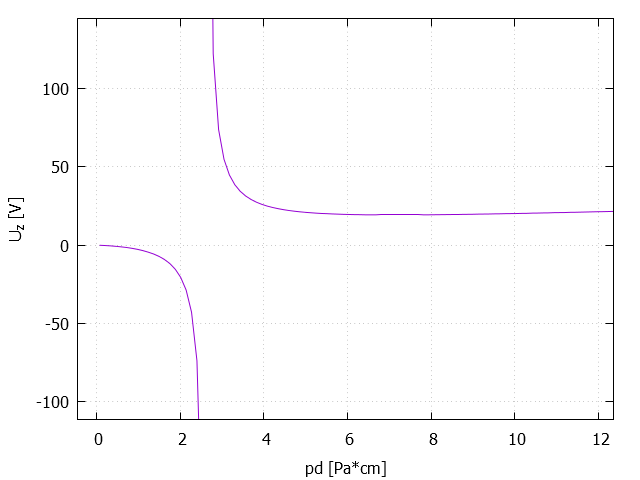
\includegraphics[width=\textwidth]{Figure/02/paschen_moje.png}
\end{minipage}
\\
\begin{minipage}[c]{200pt}
\caption{Ekvipotenciální plochy v doutnavém výboji při 100 Pa \cite{edu-techmania}.  }
\label{obr:doutnavy}
\end{minipage}
\begin{minipage}[c]{5pt}
\end{minipage}
\begin{minipage}[c]{200pt}
\caption{ Funkce f(x) je vykreslená Paschenova křivka \eqref{eq:paschen} pro hodnoty $A=2737,5$ $\frac{\text{V}}{\text{kPa} \cdot \text{cm}}$, $B=112,5$ $\frac{\text{V}}{\text{kPa} \cdot \text{cm}}$ a $\eta_+=3$.}
\label{obr:paschen_moje}
\end{minipage}
\end{figure}


\section{Přivedení vodičů k elektrodám}
\par K elektrodám, které sloužily jak pro urychlení, tak i k fokusaci elektronového svazku, jsme přiváděli jeden vodič s napětím vyšším než 20 kV a dva s napětím do 5 kV. Nejprve jsme se pokoušeli použít jedinou průchodku, u které byly všechny sousední vodiče vzdáleny méně než jeden centimetr. Podle teorie by k výboji na vzduchu mělo docházet při zhruba 20 kV/0,7 cm, což nebylo pro naše účely nedostatečné a vysoké napětí jsme přiváděli samostatnou průchodkou.
% My jsme však nebyli schopni získat z vysokonapěťového zdroje více než 5 kV pravděpodobně kvůli neúmyslnému uzemnění v jiném místě. Naším cílem bylo navíc vést vodičem více než 20 kV, čímž bychom překročili dielektrickou pevnost vzduchu. Vysoké napětí jsme tedy přiváděli samostatnou průchodkou a původní průchodkou jsme vedli pouze vodiče do 5 kV. 
\par Samostatná průchodka však nebyla uzpůsobena k vedení vysokého napětí a opět byl vodič vzdálen zhruba 1 cm od uzemněné vakuové komory. I přes naši snahu nechráněné části průchodky co nejvíce izolovat vulkanickou páskou jsme při překročení napětí 30 kV na vzduchu výboje pozorovali. Vysokonapěťovou keramicky izolovanou průchodku jsme bohužel k dispozici neměli.
\par Uvnitř komory byly jednotlivé elektrody vzdáleny od sebe navzájem a od uzemněné komory také přibližně jeden centimetr. Abychom mohli použít výpočet pomocí Paschenova zákona \eqref{eq:paschen}, je potřeba, aby podíl elektrické intenzity $E$ a tlaku $p$ byl v rozmezí $E/p=450-7500$ $\frac{\text{V}}{\text{kPa} \cdot \text{cm}}$. Námi cílený tlak byl ideálně co nejmenší, abych se náš elektronový svazek nerozptyloval na molekulách vzduchu, tedy $10^{-2}-10^{-4}$ Pa. Pro napětí $U$ v řádu kilovoltů však ze vztahu $E=U/d$ dostáváme pro $d=1$ cm $E/p \sim 10^{9}$ $\frac{\text{V}}{\text{kPa} \cdot \text{cm}}$. I kdybychom se rozhodli toto omezení nerespektovat, zjistíme, že z Paschenova zákona dostaneme pro námi zamýšlené hodnoty $p=10^{-3}$ Pa a $d=1$ cm nesmyslný výsledek $U_z<0$ \footnote{Použili jsme $A=2737,5$ $\frac{\text{V}}{\text{kPa} \cdot \text{cm}}$, $B=112,5$ $\frac{\text{V}}{\text{kPa} \cdot \text{cm}}$ a $\eta_+=3$ \cite{Bozhko}. Volba jiného $\eta_+$ v rozmezí $\eta_+=2-100$ výsledek nemění.}, jelikož má závislost \eqref{eq:paschen} průběh hyberboly (Obr. \ref{obr:paschen_moje}).
%což potvrzuje neaplikovatelnost \eqref{eq:paschen}. Jelikož má závislost \eqref{eq:paschen} průběh hyberboly (Obr. \ref{obr:paschen_moje}), je chybné se domnívat, že pro námi dosahované oblasti $10^{-4}$ Pa$\cdot$cm $\sim 8\cdot 10^{-7}$ Torr$\cdot$cm by $U_z$ šlo do nekonečna (Obr. \ref{obr:paschen_air}). 
Proto jsme neexistenci výboje v komoře odhadovali pouze na základě úvahy, že při dosaženém nízkém tlaku nebude pro výboj k dispozici dostatečný počet ionizovatelných molekul.



\section{Pozorování a diskuse}
\par Při prvních zkouškách jsme dosahovali tlaku zhruba 100 Pa a při použitém napětí 3 kV jsme pozorovali fialový doutnavý výboj (Obr. \ref{obr:fialovy_vyboj}). Naše pozorování se shoduje s očekáváním z Obr. \ref{obr:doutnavy}. Současně jsme však nepozorovali žádný signál elektronů na stínítku. Použité wolframové vlákno pravděpodobně nebylo vhodným zdrojem elektronů. 
% jako zdroje elektronů, které nám buď nedodávalo dostatečný počet elektronů, anebo jsme elektrony nebyli schopni od vlákna urychlit ke stínítku kvůli nevhodnému sestavení aparatury. 
\par Další pokusy jsme prováděli při tlaku přibližně 10$^{-2}$ Pa \footnote{Jelikož se nám ke konci semestru porouchal tlakoměr, dosažený tlak řádu 10$^{-2}$ Pa jsme odhadovali na základě alespoň třídenního čerpání vakuové komory turbomolekulární vývěvou. }. Při nich jsme již nepozorovali doutnavý výboj, ale při dosažení napětí 20 kV na urychlovací elektrodě jsme v komoře pozorovali výboje doprovázené zelenými záblesky. Pravděpodobně se jednalo o elektrony vzniklé při výboji, které dopadly na instalované fluorescenční stínítko, jelikož jsme stejné zelené světlo pozorovali na stínítku při dopadu elektronů z funkčního elektronového děla. Tyto výboje se v závislosti na použitém napětí pravidelně opakovaly a se zvyšujícím se napětím se časové intervaly mezi nimi zkracovaly. Do komory jsme viděli malým průzorem a záblesk vždy osvítil celou komoru, takže jsme ani nebyli schopni určit, kde k výbojům dochází. Výboje jsme pozorovali i v případě, kdy jsme zapojili pouze jednu elektrodu s nejvyšším urychlovacím napětím, domníváme se proto, že docházelo k výboji do komory v místě, kde byla vzdálenost elektrody od komory nejkratší. Při jednom výboji jsme dokonce pozorovali jasný jiskrový výboj (Obr. \ref{obr:jiskra}), ovšem na jiném místě.

\begin{figure}[h!]
\centering
\begin{minipage}[c]{200pt}
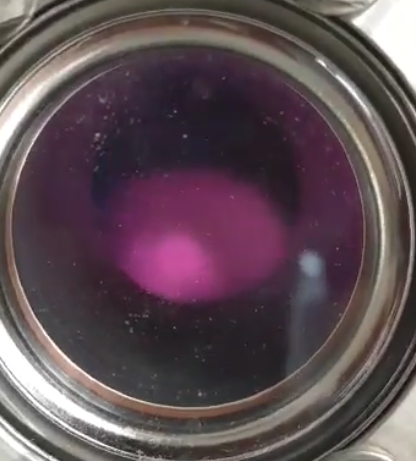
\includegraphics[width=\textwidth]{Figure/02/fialovy_vyboj.png}
\end{minipage}
\begin{minipage}[c]{200pt}
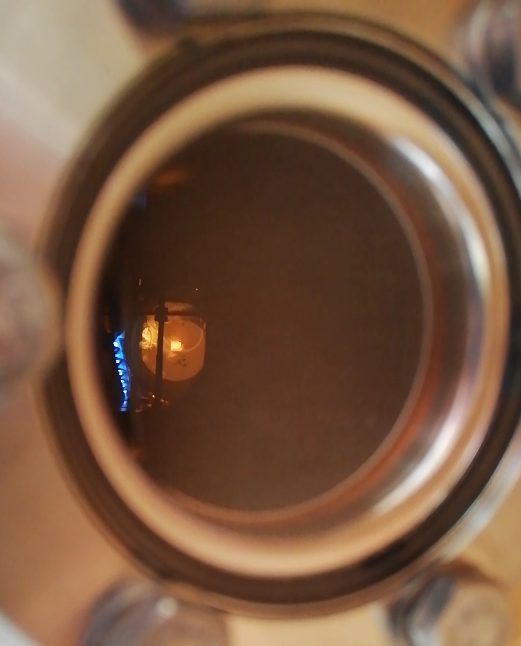
\includegraphics[width=\textwidth]{Figure/02/jiskra.png}
\end{minipage}
\\
\begin{minipage}[c]{200pt}
\caption{Pozorovaný fialový doutnavý výboj při tlaku zhruba 100 Pa.  }
\label{obr:fialovy_vyboj}
\end{minipage}
\begin{minipage}[c]{5pt}
\end{minipage}
\begin{minipage}[c]{200pt}
\caption{Pozorovaný jiskrový výboj při tlaku zhruba $10^{-2}$ Pa.}
\label{obr:jiskra}
\end{minipage}
\end{figure}


\par Při použití napětí vyššího než 30 kV jsme pozorovali výboje již u průchodky vysokého napětí z vnějšku komory na vzduchu. Výbojům jsme se snažili zabránit zvýšenou izolací vodičů vulkanickou páskou a plastovou ohebnou trubkou. Neúspěšně. Pro měření s detektorem dodaným od druhé skupiny jsme proto volili pouze urychlovací napětí do 18 kV, aby detektor výboje nepoškodily, což zkomplikovalo měření, protože jsme nedosáhli cílené energie elektronů 80 keV.
\par Navzdory našemu očekávání docházelo k výbojům ve vyčerpané vakuové komoře při nižším napětí než na vzduchu. Pro tento jev nemáme uspokojivé vysvětlení. Navíc při tlacích menších než 1,3 Pa by nemělo docházet k žádným elektrickým výbojům při jakémkoli napětí \cite{ellion}. Výboje by snad odstranilo použití keramické vysokonapěťové průchodky.

%výboje když jsme zapojili jen HV a nic jiného, výboje při 18 kV, víc jsme nepoužívali, abychom nezničili detektor



\section{Závěr}
\par K urychlení elektronů jsme se na elektrody do vakuové komory snažili přivést napětí řádu 5 kV a vysoké napětí řádu 80 kV. K vedení vysokého napětí jsme použili samostatnou průchodu, která však stejně jako původně použitá nevyhovovala podmínkám vedení vysokého napětí a při napětí vyšším než 18 kV uvnitř komory a napětí vyšším než 30 kV z vnějšku komory probíjela. Tyto hodnoty jsme proto nepřekračovali. Průchodka pro vedení napětí řádu 5 kV byla dostatečná a výboje jsme nepozorovali.
\par Navrhovaným řešením výbojů je použití keramické průchodky uzpůsobené k vedení vysokého napětí.

\newpage
\chapter{Zdroj elektronů, ES40-PS}
\label{kapTomasT}

Z důvodů problémů s nedostatkem elektronů z wolframového vlákna žárovky jsme se rozhodli k použití ES40-PS jako zdroje elektronů. ES40-PS je \textit{Electron Source Power Supply} poskytující svazek elektronů s nastavitelnou energií, hustotou, pozicí a profilem svazku. Dále umožňuje skenování oblasti s nastavitelnou rychlostí skenování. 


Schéma zapojení zdroje elektronů ES40-PS je znázorněno na Obr.~\ref{04schema} vlevo. Zdroj elektronů je upevněn pomocí průchodky do vakuové komory a připojen ke stanici ES40-PS pomocí kabelu s 6-pinovou spojkou. Na Obr.~\ref{04schema} vpravo je zobrazena ukázka ovládacího panelu stanice ES40-PS. 


\begin{figure}[htbp!]
\centering
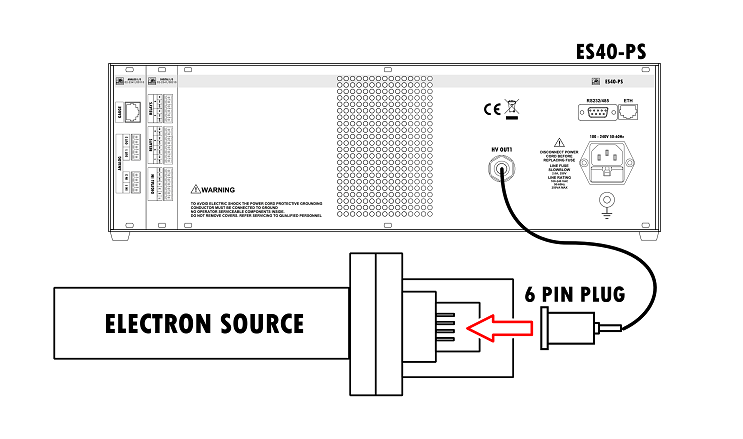
\includegraphics[width = 170 pt]{Figure/04/schema.png}
\hfill
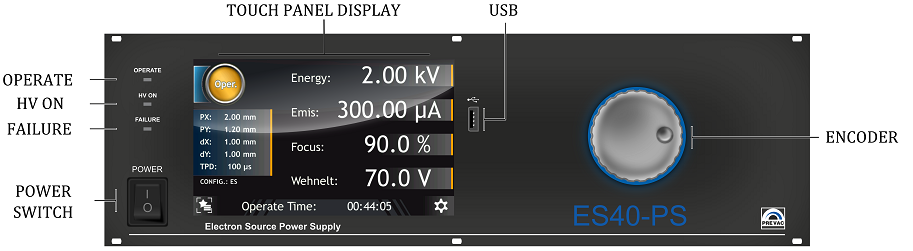
\includegraphics[width = 250 pt]{Figure/04/panel.png}
\caption[Schéma zapojení a ukázka ovládacího panelu stanice ES40-PS]{Vlevo: Schéma zapojení zdroje elektronů ES40-PS. Vpravo: Ukázka předního ovládacího panelu stanice ES40-PS. Převzato z~\cite{Manual}.}
\label{04schema}
\end{figure}

Zdroje elektronů ES40-PS má několik nastavitelných parametrů: 
\begin{itemize}
\item \textbf{Urychlovací napětí} je nastavitelné od 0 kV do 5 kV
\item \textbf{Emisní proud} elektronů je nastavitelný v rozmezí od $0{,}01 \ \mu$A do $300{,}00 \ \mu$A
\item \textbf{Fokusovací napětí} je spojené s urychlovacím a lze nastavit od 60,0 \% do 99,9 \%
\item \textbf{Wehneltovo napětí} od 0 V do 300 V
\end{itemize}
Elektrony vychází ze zahřívání wolframové katody, z tohoto důvodu se může objevit zpráva "Current Limit", kdy je zapotřebí více času ke stabilizaci emisního proudu. 

Zmíněné hodnoty je možné nastavit na úvodní obrazovce ovládacího panelu viz Obr.~\ref{04display}. Po kliknutí na zmenšený seznam hodnot nacházející se v levé části se display přepne do druhé polohy, kde je možné nastavit následující hodnoty:
\begin{itemize}
\item \textbf{Horizontální výchylka} PX je nastavitelná v rozmezí od $-5{,}00$ mm do $5{,}00$ mm 
\item \textbf{Vertikální výchylka} PY je nastavitelná v rozmezí od $-5{,}00$ mm do $5{,}00$ mm 
\item \textbf{Horizontální rozsah skenu} dX je nastavitelný v rozmezí od $0{,}00$ mm do $10{,}00$ mm
\item \textbf{Vertikální rozsah skenu} dY je nastavitelný v rozmezí od $0{,}00$ mm do $10{,}00$ mm
\item \textbf{TPD hodnota} (\textit{time per dot}) je nastavitelný v rozmezí od $20 \ \mu$s  do $30$ ms
\end{itemize}

Všechny výše uvedené parametry byly otestovaný a jejich vliv na elektronový svazek byl změřen a je popsán v sekci \ref{TestDela}.

Při současném nastavení výchylky a skenu se může objevit zpráva "SCAN X/Y OVERFLOW", která značí překročení fyzikálního rozsahu zdroje elektronů ES40-PS a pro její odstranění je nutné snížit výchylku svazku nebo rozsah skenování. 

\begin{figure}[htbp!]
\centering
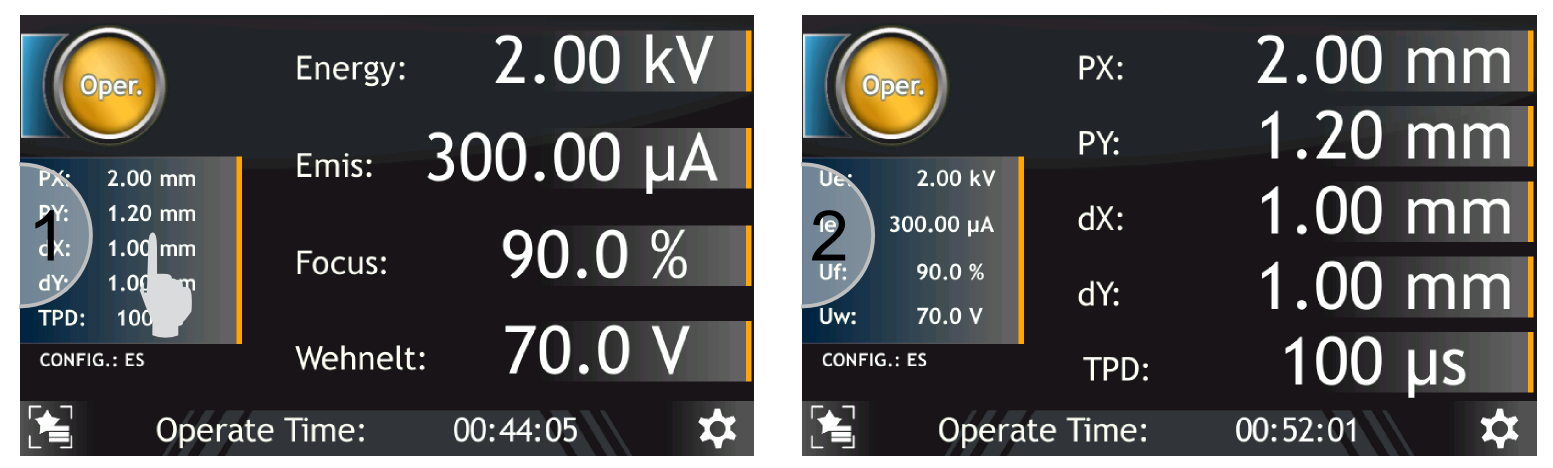
\includegraphics[width = 370 pt]{Figure/04/display.png}
\caption[Ukázka nastavení parametrů zdroje elektronů]{Ukázka nastavení parametrů zdroje elektronů a přepnutí do druhého menu. Převzato z~\cite{Manual}}
\label{04display}
\end{figure}

%princip změny polohy?
%
%\begin{figure}[htbp!]
%\centering
%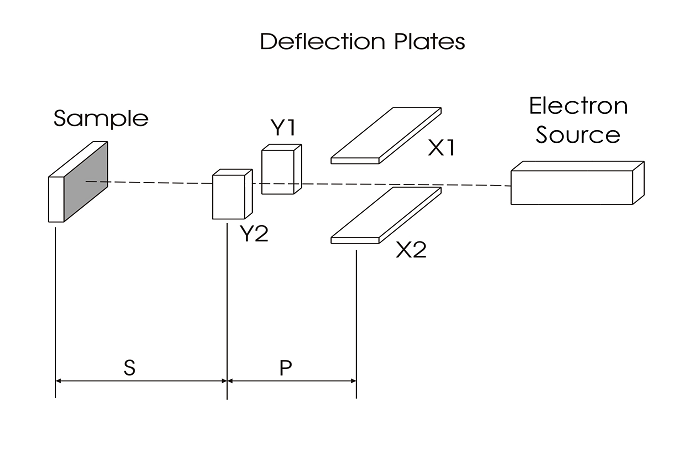
\includegraphics[width = 170 pt]{Figure/04/schema2.png}
%\caption{. Převzato z~\cite{Manual}}
%\label{04schema2}
%\end{figure}

Spuštění zdroje elektronů ES40-PS krok za krokem:
\begin{enumerate}
\item Po zapnutí napájení by měl být zdroj ponechán v režimu \textit{STAND-BY} alespoň 10 minut pro řádné zahřátí a stabilizaci katody
\item Pokud zdroj nebyl použit delší dobu následuje \textit{DEGAS} procedura
\item Následuje zapnutí do \textit{OPERATE} módu, ale pouze v případě je-li tlak v komoře nižší než $5 \times 10^{-6}$ mbar
\item Doporučené začínající hodnoty jsou: Energie = 3 kV, Emise = 100 $\mu$A, Fokusace = 70 \%, Wehneltovo napětí = 85 V, PX = PY = dX = dY = 0 mm
\end{enumerate} 


\textbf{DEGAS} procedura:
\begin{enumerate}
\item Před zapnutím do \textit{OPERATE} módu je nutné nastavit všechny napětí a proudy na minimum. 
\item Po zapnutí do \textit{OPERATE} módu je nutné nastavit následující parametry v daném pořadí: Energie = $2{,}00$ kV, Fokusace = $88{,}0$ \% a Wehneltovo napětí~=~$71{,}0$~V
\item Zvýšení Emise na $300{,}00 \ \mu$A 
\item S tímto nastavením by mělo zařízení pracovat 10 minut
\item Následně by měla být emise snížena na minimum a poté i zbývající napětí
\end{enumerate}
Během \textit{DEGAS} procedury by měly být parametry zvyšovány postupně se současnou kontrolou tlaku v komoře. Pokud dojde k náhlému poklesu vakua v komoře, mělo by být zařízení ponecháno se stávajícími parametry dokud nedojde k obnovení vakua.

Více podrobností k ovládání zdroje elektronů ES40-PS je popsáno v operačním manuálu ~\cite{Manual}.

\newcommand{\fig}[3]{ 
	\begin{figure}[!ht]
		\centering
		\includegraphics[width=#1\linewidth]{Figure/05/#2.png}
		\caption{#3}
		\label{#2}
	\end{figure}
}

\interfootnotelinepenalty=10000
\renewcommand{\figurename}{Obr.}
\newcommand{\figref}[1]{\figurename \hspace{1 pt} \ref{#1}}

\newpage \clearpage

\chapter{Detekce}

\section{Detekční technologie}
Po zvážení možností způsobu detekce elektronového svazku bylo jako optimální možnost zvoleno použití křemíkového pixelového detektoru X-CHIP03 vyvinutého v rámci FJFI ČVUT v Praze skupinou CAPADS. Ten by měl, jakožto detektor ionizujícího záření, dobře posloužit účelu, tedy zaznamenávání průletu elektronů. Další výhodou jeho použití byla možnost konzultace s týmem, který jej vytvořil. 

Vzhledem k monolitické technologii, v níž je detekční čip navržen, existuje spodní hranice pro energii detekovaných částic. Ta byla pro elektrony ze simulací stanovena na 60 keV - hodnotu, jíž bylo teoreticky elektronovým dělem dosáhnout. Vzhledem ke komplikacím, které se objevily během testování (dříve zmíněné vakuové výboje, ...) se nakonec bohužel podařilo dosáhnout energií maximálně 15 keV, které neprojdou vrstvou elektroniky do citlivé oblasti.

K vyřešení tohoto problému bylo navrženo využití konverzní vrstvy slitiny mědi a zlata. Tato tenká folie byla umístěna do cesty svazku před detektorem a při ozařování elektrony docházelo k emisi fotonů o podobné energii, které už nebyl problém detekovat. 

\section{Principy polovodičových detektorů}
\subsection{Pásová struktura}
Krystalické pevné látky se klasifikují jako vodiče, polovodiče a izolanty, přičemž kriteriem pro toto rozdělení je tzv. šířka zakázaného pásu. Ta vyplývá z pásové struktury (\figref{pasova_struktura}), tedy modelu, který popisuje energetické rozdělení elektronů v krystalu. 

\fig{1}{pasova_struktura}{Grafické znázornění pásové struktury a) izolantu, b) polovodiče a c) vodiče. \cite{lutz1999semiconductor}}

Energetické spektrum samostatného elektronu je diskrétní, přičemž jednotlivé hladiny jsou určeny kvantovými čísly. Přidáváním dalších elektronů postupně dochází k rozštěpení hladin a při přechodu k makroskopickému popisu krystalu, je již třeba použít statistický model. Tím je pásová struktura, ve které se při velkém počtu elektronů původně diskrétní energetické hladiny shlukují do spojitých pásů - valenčního a vodivostního.

\textit{Valenční pás} obsahuje energie, při kterých jsou elektrony vázané v atomovém obalu a nemohou se volně pohybovat látkou. 

Přijme-li elektron dostatečnou energii, může přejít do \textit{vodivostního pásu}, ve kterém je v rámci krystalické mřížky delokalizovaný a může se podílet na vedení elektrického proudu.

Je-li krystalická látka vodivá, oba tyto pásy se překrývají a elektrony se tak mohou podílet na vedení proudu přirozeně. 

V případě izolantů jsou naopak pásy oddělené širokou oblastí energií, kterých elektrony nemohou nabývat - tzv. zakázaným pásem. Jeho šířka v prvním přiblížení\footnote{Roli zde hrají ještě další faktory, které oproti samotné ionizační energii šířku pásu zvětšují.} odpovídá ionizační energii atomů. 

Polovodiče mají sice ve své struktuře zakázaný pás také, jeho šířka je však na rozdíl od izolantů menší (řádově v jednotkách eV). To umožňuje korigovat jejich vlastnosti tak, aby podle potřeby vedly nebo nevedly elektrický proud. Když dojde k ionizaci atomu, vytvoří se v polovodiči dva efektivní nosiče náboje. Elektrony, které jsou na \figref{pasova_struktura} zobrazeny tečkami ve vodivostním pásu a díry, tedy absence elektronů v páse valenčním, zobrazené prázdnými kroužky.

Pohyb elektronů a děr společně vytváří celkový proud, přičemž elektrony se v materiálu pohybují rychleji\footnote{V křemíku je mobilita elektronů oproti děrám $\sim 3 \times$ větší.}.

\subsection{Vyprázdněná oblast}
Vlastnosti polovodičů mohou být zlepšeny tzv. dopováním. Při tomto procesu dochází k nahrazení malého množství atomů původní látky atomy s jiným (ale velmi blízkým) protonovým číslem. Tím vznikne přebytek nebo naopak nedostatek elektronů v krystalové mřížce\footnote{Polovodiče typu N mají přebytek elektronů, typu P přebytek děr.} a jsou tak apriori přítomny volné nosiče náboje.

Připojíme-li k sobe opačně dopované polovodiče, vznikne dioda a na jejím rozhraní tzv. vyprázdněná oblast, viz \figref{depleted}. Jde o místo, ze kterého jsou volné nosiče náboje vypuzeny vlivem přirozeně vzniklého elektrického pole. Pokud je navíc na diodu přivedeno napětí v závěrném směru, šířka vyprázdněné oblasti se zvětší.

\fig{.9}{depleted}{Přechod mezi P (nalevo) a N (napravo) polovodiči. Znaménka v kroužku značí volné nosiče náboje, které jsou v přítomnosti pole odpuzeny, nezakroužkovaná znaménka pak ionty ve vrcholech krystalické mřížky. Graf pod obrázkem zobrazuje průběh odpovídajícího potenciálu. \cite{spieler2005semiconductor_detector_systems}}

%Základním prvkem polovodičového detektoru je tzv. vyprázdněná oblast. Jde o místo s minimální koncentrací volných nosičů náboje, které vznikne v diodě při jejím zapojení v závěrném směru, viz \figref{depleted}. Na diodu je dále přivedeno tzv. biasovací napětí, které dále rozšiřuje vyprázdněnou oblast a navíc urychluje volné nosiče náboje, které by v ní vznikly.

\subsection{Vznik signálu}
%Pakliže vyprázdněnou oblastí proletí ionizující částice, předávají energii vázaným elektronům, které přejdou do vodivostního pásu. Při tomto přechodu vzniknou dva volné nosiče náboje: volný elektron a tzv. díra, tedy vakance ve valenčním páse, která se efektivně chová jako volný nosič náboje opačného znaménka. 

Pokud proletí elektricky nabitá částice vyprázdněnou oblastí předávají energii vázaným elektronům. Tak může dojít k předání energie dostatečné k přechodu vázaného elektronu do vodivostního pásu, tedy ionizaci atomu. Tím vznikne elektron-děrový pár.

Pokud má částice dostatečnou energii, mohou tyto páry vznikat podél celé její trajektorie, jak je vidět na \figref{particle-detection}. V elektrickém poli\footnote{Pole vzniká jako přirozený důsledek závěrného zapojení diody v kombinaci s biasovacím napětím.} driftují směrem ke sběrným elektrodám, které mohou bít umístěny na přední a zadní straně senzitivní oblasti.

Driftem elektronů a děr vzniká v materiálu proud, který je následně registrován jako signál. Jeho časový vývoj závisí například na typu nosiče\footnote{Elektrony se v křemíku pohybují $\sim 3 \times$ rychleji, než díry.} nebo na jeho aktuální poloze, pak záleží na tvaru elektrického pole v souladu se Shockley-Ramovým teorémem \cite{ramo1939}, \cite{shockley1938}. Příklad časové závislosti signálu je na \figref{pd_weightfield_mu}.

\fig{1}{particle-detection}{Znázornění elektron-děrových párů vzniklých ve vyprázdněné oblasti detektoru při průletu různých druhů ionizujících částic.}

\fig{1}{pd_weightfield_mu}{Časový vývoj proudového signálu generovaného mionem o energii 1 GeV v pixelu křemíkového. Model z programu Weightfield2 \cite{2015weightfield}. Oranžová křivka značí proud indukovaný pohybem děr,modrá pohybem elektronů a černá celkový.}

\clearpage

\section{Pixelové detektory}
Polovodičové detektory se podle strukrtury uspořádání senzitivních oblastí dělí na stripové a pixelové. 

U prvních zmíněných je senzitivní oblast rozdělena na proužky (stripy), což je technologicky snazší varianta, detektor ale tak poskytuje informaci o zásahu pouze v jednom rozměru. 

Pixelové detektory naproti tomu mají senzitivní oblast tvořenou maticí pixelů, díky čemuž je jejich prostorové rozlišení apriori dvourozměrné. Pro účely skenování průřezu svazku je tedy pixelový detektor ideální volbou. Navíc se nabídla možnost využití pixelových detektorů vyvíjených na katedře, díky čemuž bylo možné v průběhu práce konzultovat jejich aplikaci s designéry.

V průběhu práce na experimentu se bohužel ukázalo, že výhody 2-D rozlišení není možné dostatečně využít, protože se nepodařilo svazek fokusovat do dostatečně malého průřezu a detektor tak vždy snímal pouze jeho část. Volbu pixelového detektoru však přesto považujeme vzhledem k detektoru za nejlepší možnou variantu.

%Jedním z typů polovodičových detektorů jsou pixelové, tedy matice nezávislých detekčních jednotek. Oproti druhé nejvýznamnější rodině - stripovým - nabízí apriori 2D rozlišení což je pro účel příčného skenování  elektronového svazku ideální. Tato potenciální výhoda bohužel nakonec zůstala nevyužita, protože se nepodařilo svazek dostatečně fokusovat a v místě detekce tak pokrýval větší plochu, než samotný detektor.\footnote{Je také možné, že k defokusaci svazku došlo využitím konverzní vrstvy.}

\section{X-CHIP03}
Pro skenování elektronového svazku byl v rámci tohoto projektu zvolen X-CHIP03 (\figref{xchip03_mp}). Jde o monolitický\footnote{V případě monolitických detektorů je na rozdíl od hybridních vyčítací část elektroniky umístěna ve stejném jednolitém objemu křemíku jako senzitivní vyprázdněná oblast.} pixelový detektor tvořený maticí 64x64 pixelů o rozměrech $4.2\times 5 \mathrm{mm}^2$. 

\fig{1}{xchip03_mp}{Model designu (vlevo) a fotografie (vpravo) detekčního čipu X-CHIP03, \cite{xchip03}.}

Detekční set-up, viz \figref{setup} se skládá z čipu umístěného na FURRy, PCB zprostředkující transfer fyzického signálu do USB portu, který je možné přímo připojit k počítači. Ke zpracování dat pak slouží software ASPIRE, přičemž obě zmíněné složky byly vyvinuty v rámci CAPADS. Celý set-up je umístěn na stojanu, který byl pro tento účel navržen a vytvořen ve 3-D tiskárně. Přechod mezi vakuem a notebookem vyčítajícím data byl zajištěn přes přechodku vakuové komory, na kterou byl z obou stran zajištěn rozpojený USB kabel.

\fig{1}{setup}{Experimentální detekční set-up. V pravé části se nachází detekční čip X-CHIP03, překrytý zlatavou konverzní folií. Větší PCB je FURRy, oranžové komponenty slouží jako stojánek, dále upevněný ve vakuové komoře. Z levé části rovněž vystupuje port USB.}

\label{chapter2}

\clearpage \pagebreak \newpage

\chapter*{Shrnutí}
\addcontentsline{toc}{chapter}{Shrnutí}

\clearpage 
\addcontentsline{toc}{chapter}{Reference} 


\bibliography{bibliografie}{}
\bibliographystyle{ieeetr}

\end{document}